\documentclass[crop,tikz]{standalone}% 'crop' is the default for v1.0, before it was 'preview'
%\usetikzlibrary{...}% tikz package already loaded by 'tikz' option
\usetikzlibrary{decorations.pathreplacing}
\begin{document}
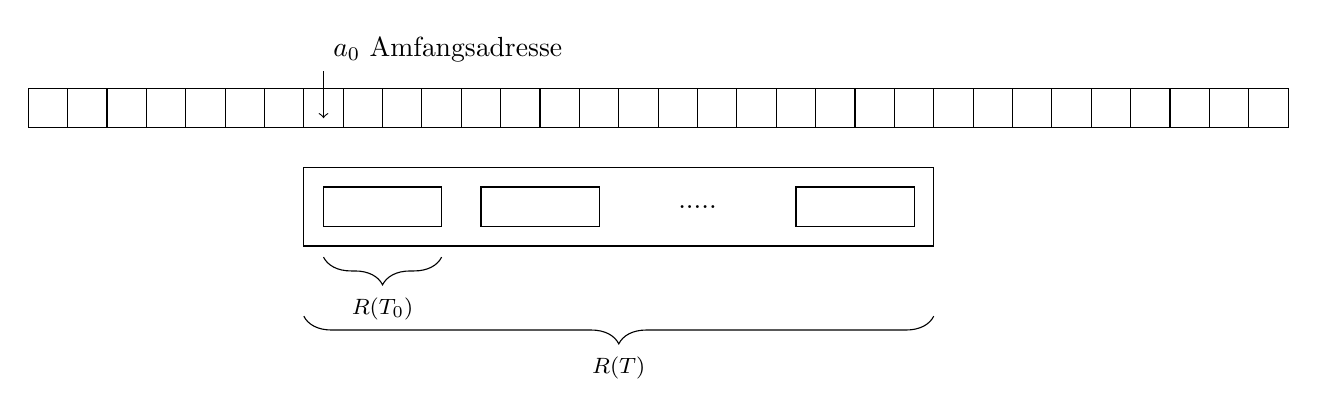
\begin{tikzpicture}
\foreach \i in {0.5,1.0,...,16}{
	\draw [] (\i,0) rectangle (\i+0.5,0.5);
	}
	
\node [anchor=west] (A) at (4.25, 1) {$a_0$ Amfangsadresse};
\node [anchor=west] (B) at (4.25, 0) {};
%\node [minimum height=.5] (c) at (8.25, -1.25) {Test...};

\draw [->] (A.south west) -- (B.north west);

\draw [] (4,-.5) rectangle (12,-1.5);
\draw [] (4.25,-.75) rectangle (5.75,-1.25);
\draw [] (6.25,-.75) rectangle (7.75,-1.25);
\draw [] (10.25,-.75) rectangle (11.75,-1.25);
\fill [white] [align=center] (8.25, -.75) rectangle (9.75,-1.25)  node[pos=.5, color=black] {.....};
\draw [decorate,decoration={brace,amplitude=10pt,mirror,raise=4pt},yshift=0pt]
(4.25,-1.5) -- (5.75,-1.5) node [black,midway,yshift=-0.8cm] {\footnotesize $R(T_0)$};
\draw [decorate,decoration={brace,amplitude=10pt,mirror,raise=4pt},yshift=0pt]
(4,-2.25) -- (12,-2.25) node [black,midway,yshift=-0.8cm] {\footnotesize $R(T)$};


\end{tikzpicture}

\end{document}
